\section{Journey Analysis}
\label{sec:journeyanalysis}
\subsection{Time of Movement}
\label{sec:timeofmovement}

To find patterns in the time of employees’ movements a graph showing when an employee moved is plotted. The time in Figure \ref{fig:MoveTime} begins at the time of the first GPS data point. If an employee moves during an hour a point is plotted. The colour of the marker indicates the employees current employment type. Yellow indicates an information technology worker, blue indicates an engineer, red indicates an executive, cyan indicates a security worker and green indicates a truck driver.   

\begin{figure}[H]
\centering
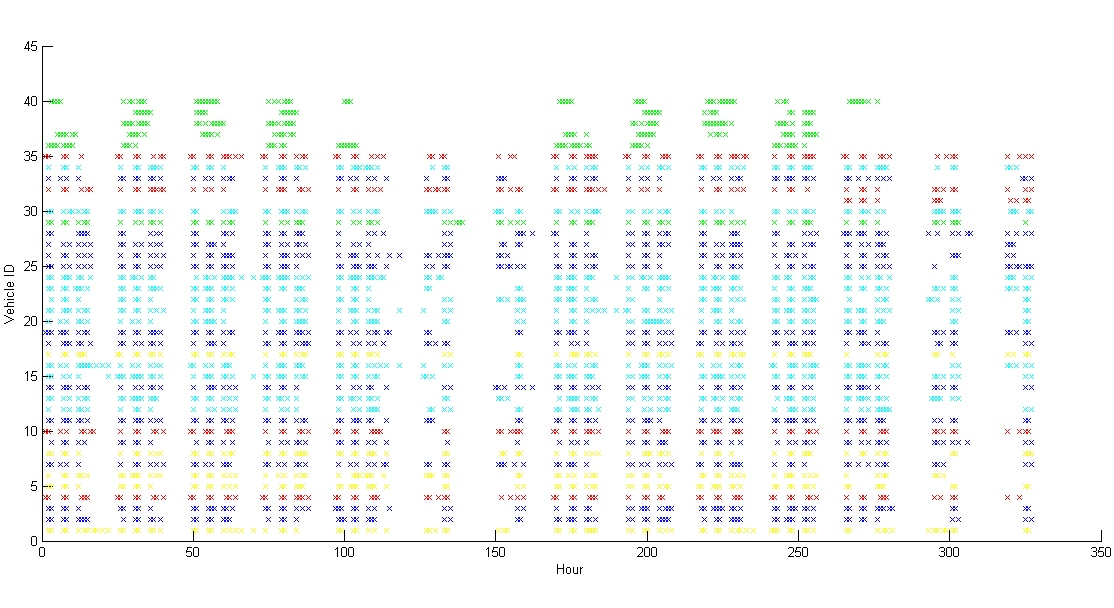
\includegraphics[width=1.2\textwidth]{MoveTime.jpg}
\caption{\label{fig:MoveTime}A data point shows a vehicle ID moved in that hour.}
\end{figure}


\noindent Figure \ref{fig:MoveTime} shows a number of interesting patterns. Most employees move during the day and then have a period overnight when they don’t move, as expected. However, it can be seen that some employees move in the day, then continue to move when most other employees stop. There are five employees showing this unusual pattern in their movements, they are identified in table \ref{table:time_ids}. \\


\begin{table}[H]
\begin{center}
\begin{tabular}{|l|l|l|}
\hline
Vehicle ID & First Name & Last Name \\ \hline \hline

1 &Lucas & Alcazar\\ \hline
15&Loreto&Bodrogi\\ \hline
16&Isia& Vann\\ \hline
21&Hennie&Osvaldo \\ \hline
24&Minke& Mies

\end{tabular}
\caption{\label{table:time_ids}Employees showing unusual patterns in their movement.}
\end{center}
\end{table}

\noindent To investigate this behaviour the tracking data for each employee is split into individual journeys to give an insight into where these employees are travelling. A journey enda if a vehicle does not move for more than 10 minutes. When these journeys are plotted, as shown in Figure \ref{fig:TimeJourneys},  it can be seen that vehicles 15, 16, 21 and 24 all start in a similar area and make very similar journeys. Vehicle 1 appears to make a set of journeys that are independent of the other 4 vehicles, so these patterns are considered as 2 different anomalies. 

\begin{figure}[H]
\centering
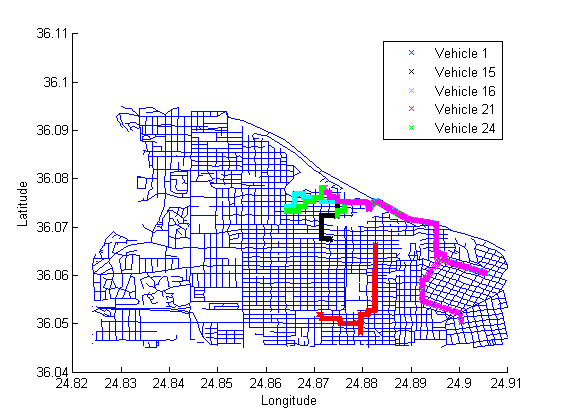
\includegraphics[width=0.9\textwidth]{TimeJourneys.png}
\caption{\label{fig:TimeJourneys}The journeys made at unusual times.}
\end{figure}

\subsection{Clustering Journeys}
\label{sec:clusteringjourneys}

\noindent To see locations frequently visited, clustering is applied to the start and end points of the journeys. Agglomerative hierarchical clustering is used, this is preferred to k-means clustering as the number of clusters in the data is unknown. Figure \ref{fig:Clustering} shows the clusters found that contain 5 or more data points. The threshold is set at 5 data points as this removes the small clusters and leaves the most frequently visited clusters. Most locations with credit card transactions have a large cluster around them, and there is also a large cluster around what is believed to be the Gastech office. There are also clusters that appear to be the homes of the employees, they are usually visited by one employee and are the last place visited at the end of the day. \\

\begin{figure}[H]
\centering
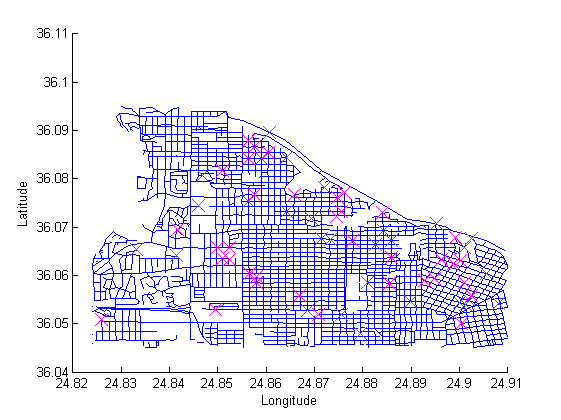
\includegraphics[width=1.1\textwidth]{Clustering.png}
\caption{\label{fig:Clustering}Clusters with 5 or more data points found using agglomerative hierarchical clustering.}
\end{figure}

\noindent When comparing these clusters to the unusual journeys it is seen that all of these unusual journeys start and end at a cluster. The first night of unusual activity by vehicle 1 shows the employee travelling from their home to the office and then back to their home. On the second night of unusual behaviour the employee travels from an establishment identified as Ouzeri Elian, to the office and then to their home. This doesn’t match the behaviour of any other employee and is consider as an anomaly.\\

\noindent Vehicles 15, 16 and 21 all start their unusual journeys from the same cluster, there are no establishments at this location and it is not known what is there. This cluster is also visited by one other employee in vehicle 13. Vehicle 24 starts from a different cluster, again there are no establishments at this location, this cluster is also visited by vehicles 17 and 33. The vehicles then travel to 4 different clusters, each of these clusters is visited by 3 different people, 2 from the set of employees being investigated and one executive. On further investigation it appears these clusters are the executives’ homes as they are regularly visited by the executive and are the last place visited at the end of the day. Table \ref{table:watch_table} shows a summary of these visits.


\begin{table}[H]
\begin{center}
\begin{tabular}{|l|l|l|}
\hline
Executive & First Employee & Second Employee \\ \hline \hline

Ingrid Barranco &Loreto Bodrogi &Isia Vann \\ \hline
Ada Campo-Corrente&Loreto Bodrogi&Minke Mies\\ \hline
Orhan Strum&Isia Vann& Hennie Osvaldo\\ \hline
Willem Vasco-Pais&Hennie Osvaldo& Minke Mies\\ \hline
\hline

\end{tabular}
\caption{\label{table:watch_table}A summary of employees at exectives' houses.}
\end{center}
\end{table}


\noindent To find any further connection between the four employees being investigated and the three employees that appeared at the start points of the unusual journeys all clusters visited by three or more of the employees being investigated are found. Five clusters are found that contain only a subset of the employees being investigated as well as Inga Ferro in vehicle 13, as shown in Figure \ref{fig:Watch_Clusters}. This suggests that there is a connection between Inga Ferro and the other employees being investigated. There appears to be no further connection between vehicles 17, 33 and the employees being investigated as there are no additional clusters containing a subset of the employees being investigated and these vehicles. 

\begin{figure}[H]
\centering
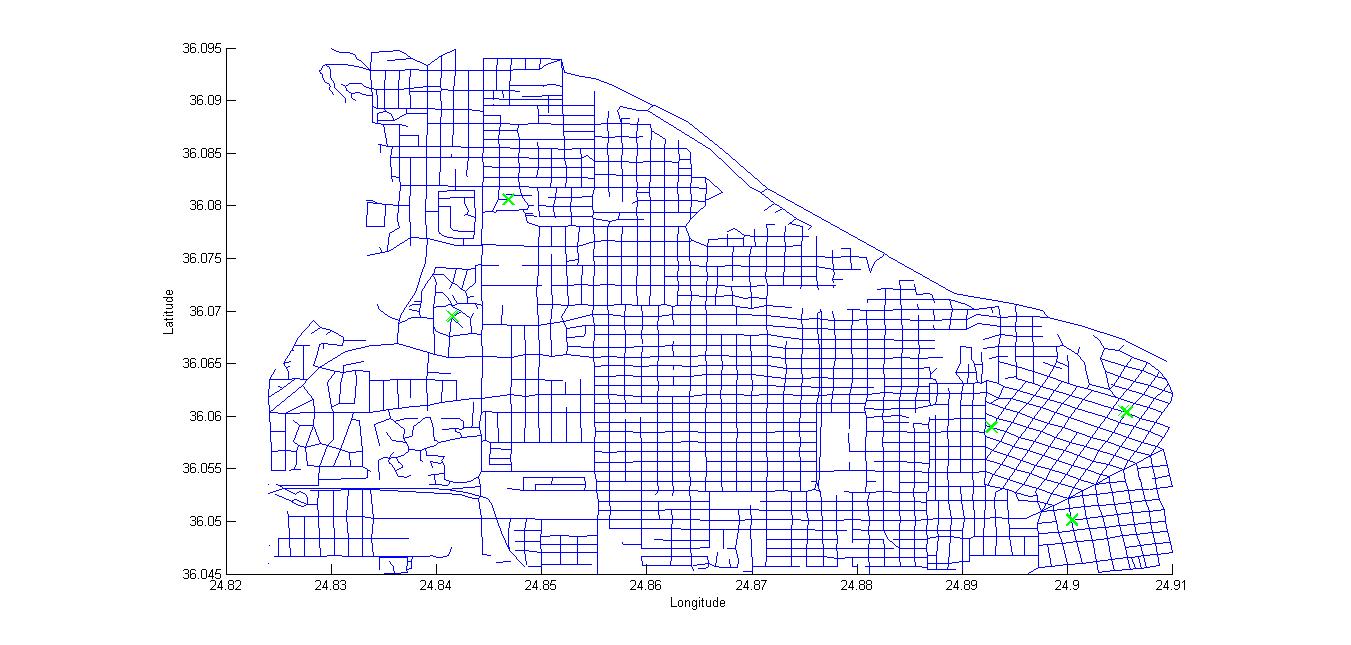
\includegraphics[width=0.9\textwidth]{Watch_Clusters.png}
\caption{\label{fig:Watch_Clusters}Clusters only visited by a subset of the suspect individuals.}
\end{figure}

\noindent To continue on the results in section 4 clusters visited by Elsa Orilla are investigated. It is discovered that Elsa Orilla in vehicle 28 uniquely visits 4 clusters.  These clusters are shown in Figure\ref{fig:ID28_Clusters}, there are no known establishments at these locations. 

\begin{figure}[H]
\centering
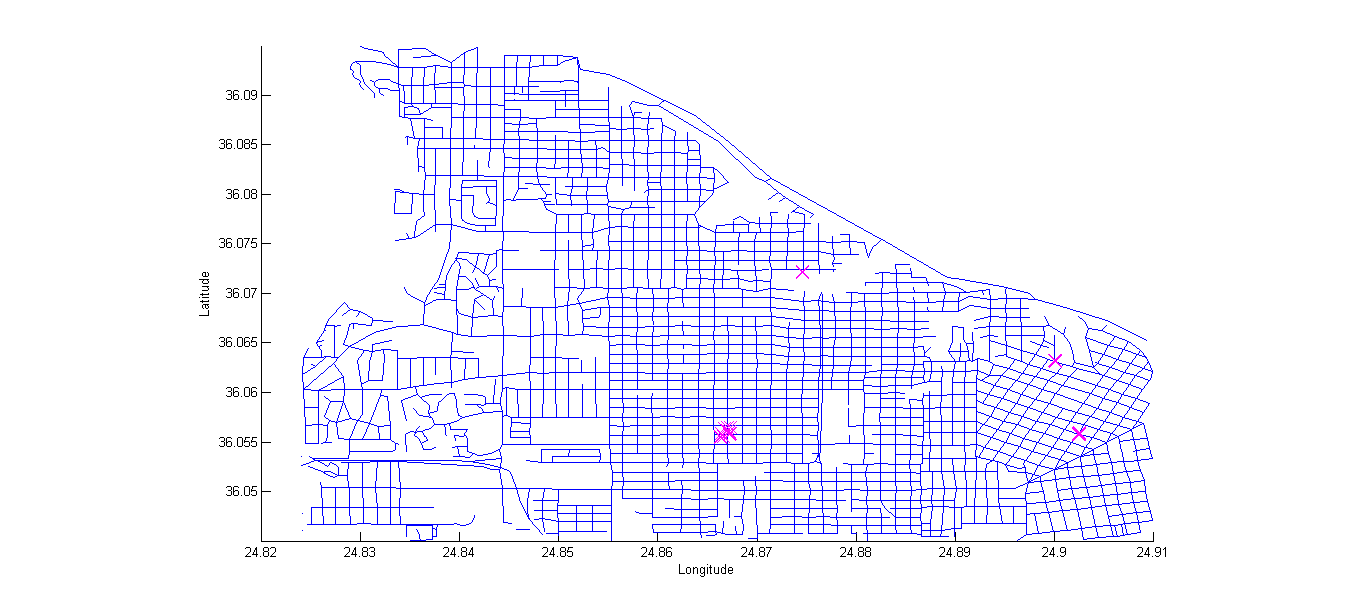
\includegraphics[width=0.9\textwidth]{ID28_Clusters.png}
\caption{\label{fig:ID28_Clusters}Clusters only visited by Elsa Orilla.}
\end{figure}


